\chapter{Concepts: Thermalization and absence thereof in closed quantum systems}\label{ch:concepts-thermalization}

%In Part 1 of this thesis, we study thermalization and localization in closed quantum systems. Specifically, we consider the paradigmatic Heisenberg quantum spin model where the couplings between the spins arise from power-law interactions among randomly placed spins. This class of models arises in many physical systems with dipolar/electronic interactions such as e.g. cold atoms, polar molecules and NV centers in diamond.\FIXME{some citations}

%This chapter starts by giving an introduction in the concepts underlying thermalization in closed quantum systems (Section~\ref{sec:Thermalization-in-closed-QS}). We then discuss many-body localization (MBL) highlighting the current understanding in the literature with a specific focused on localization in bond-disordered and long-range systems (Section~\ref{sec:MBL}). Finally, we close this chapter with a short introduction of the Rydberg experiment that we use for motivating the model we study throughout this part (Section~\ref{sec:Rydberg-experiment}).

%\FIXME{roter Faden: These concepts are useful for the description/understanding of large quantum systems! Also revise high-level introduction with this in mind.}

In this chapter, we give a brief overview of the concepts relevant for Part~\ref{pt:spatial-disorder} of this thesis and establish the necessary context to interpret the results. However, we'll try to be brief and only summarize the essence of the matter. The interested reader is referred to the relevant literature for the details.
Since the distinction between thermalizing and localized systems is at the core of this part of the thesis, we start by reviewing the current understanding of the thermalization process in closed quantum systems in general and contrast this with the typical picture of how localized systems evade thermalization. In particular, we discuss localization in long-range and bond-disordered systems. We close this chapter with a high-level description of the Rydberg-based quantum simulation experiment which naturally implements the specific disordered Hamiltonian studied here.

\section{Thermalization in closed quantum systems}
\label{sec:Thermalization-in-closed-QS}
The simplest picture of thermalization in a classical system is perhaps the gas in a box which initially is confined to one of the sides (cf. \autoref{fig:gas-in-box}). Upon removing the constraint, the gas quickly spreads throughout the box and soon after a new equilibrium is reached. Interestingly, we can understand this process in a purely statistical way, without knowing about the precise equations of motion. As long as the dynamics sufficiently explore the configuration space, i.e. are \emph{ergodic}, we can postulate each possible configuration to be equally likely. This already explains why we find the gas to distribute itself throughout the box: There are just overwhelmingly more configurations where the particles occupy most of the box than configurations where the particles are concentrated, i.e. most configurations are \emph{typical}. With this ansatz, we could also compute how much force we would need on average to slowly compress the gas back to one side and how much kinetic energy this process adds. Thus the presence of a thermal equilibrium grants us enormous predictive power.
The key features of a thermal equilibrium are:
\begin{itemize}
	\item \emph{Loss of memory}: One cannot tell on which side of the box the gas started.
	\item \emph{Subsystem independence}: Every patch of space appears to be thermal with the same parameters (at least sufficiently away from the boundary).
	\item \emph{Independence of microscopic details}: The full state of the system can be described using just a few macroscopic quantities, namely in this case the total (kinetic) energy, the number of particles and the volume of the box.
\end{itemize}

\begin{figure}[htb]
	\centering
	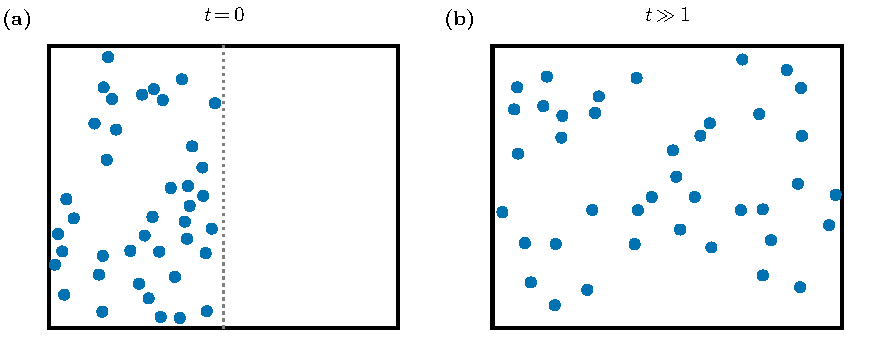
\includegraphics[]{gfx/part1/gas-in-box}
	\caption{Gas in box. (a) Initially all particles are confined to the left. (b) At a later time the gas has spread evenly throughout the box.}
	\label{fig:gas-in-box}
\end{figure}

Since quantum systems become computationally intractable much faster than classical systems, it would be very helpful if such an approach could be applied as well. Fortunately, for many quantum systems an analogue to classical thermalization can indeed by found, which we can only sketch here.
%However, the precise conditions under which a quantum system reaches thermal equilibrium are not fully understood and so one needs to check the validity of thermal descriptions on a case-by-case basis.
We refer the interested reader to one of the many great reviews on this topic for further details~\cite{gogolinEquilibrationThermalisationEmergence2016,dalessioQuantumChaosEigenstate2016,deutschEigenstateThermalizationHypothesis2018,moriThermalizationPrethermalizationIsolated2018}.

Consider some quantum system governed by a Hamiltonian $H$ which is prepared in some pure state $\ket{\psi(t)}=\ket{\psi_0}$ at $t=0$. Written in the energy eigenbasis $H\ket{k}=E_k\ket{k}$, the state at some later time $t$ can be written as
\begin{equation}
	\ket{\psi(t)} = e^{-iHt}\ket{\psi_0} = \sum_k e^{-iE_kt}\ket{k}\braket{k}{\psi_0}	= \sum_k c_k e^{-iE_kt}\ket{k}.
\end{equation}
Notably, due to the unitarity of the time evolution, the system's state at every time $t$ can be reversed to $t=0$ and thus the memory of the initial state is always preserved perfectly. This basic fact already means that we cannot expect \emph{every} observable to be captured by a thermal description of a few parameters.

However, in practice it is impossible to measure e.g. the expectation value of some projector onto a highly-entangled, many-body state. Thus for practical applications it would be sufficient, if the expectation values of some \emph{simple observables} could be described by thermal ensembles. So suppose
we restrict ourselves to measuring the expectation value of some \emph{local observable} $O$ which only acts on a small subsystem $S$, i.e. can be written as $O=O_S\otimes \bbone_{\bar{S}}$. Writing out the evolution of the expectation value, we see
\begin{align}
	\braket[1]{O(t)} &= \braket[3]{\psi(t)}{O}{\psi(t)} \\
	& = \Tr (O_S\otimes\bbone_{\bar{S}})\ketbra{\psi(t)}{\psi(t)}\\
	& = \Tr O_S \Tr_{\bar S} \ketbra{\psi(t)}{\psi(t)}\\
	&= \Tr O_S \rho_S(t).
\end{align}
So the fact alone that we measure a property $O$ on a subsystem makes this measurement effectively equivalent to measuring $O$ on a mixed state! This simple observation is what enables equilibration and thermalization of local observables. Indeed, it has been shown that such a reduced state $\rho_S(t)$ is close to its equilibrium state
\begin{align}
	\omega_S &= \lim_{\tau\rightarrow\infty}\int_{0}^{\tau}\!\mathrm{d}t \Tr_{\bar S}\rho(t)\\
	&= \Tr_{\bar S} \sum_k |c_k|^2 \ketbra{k}{k}\\
	&= \Tr_{\bar S} \omega
\end{align}\label{eq:diagonal-ensemble}
for most times $t$ under very mild conditions~\cite{reimannFoundationStatisticalMechanics2008,lindenQuantumMechanicalEvolution2009}. 
The equilibration to this so-called diagonal ensemble $\omega$ is not yet equivalent to thermalization~\cite{dziarmagaDynamicsQuantumPhase2010,polkovnikovColloquiumNonequilibriumDynamics2011}. For one $\omega$ still requires knowledge of an extensive amount of eigenstates occupation numbers  $|c_k|^2$ and additionally the system might take very long to equilibrate as the derivation relies on the dephasing of off-diagonal elements. So in the worst case, equilibration takes up until $t_{deph} \propto 1/\delta$ where $\delta=\min_{k,k'}|E_k-E_{k'}|$ is the smallest energy gap of the Hamiltonian which generally shrinks exponentially with increasing system size. 

To ensure thermalization additional assumptions are required. Considering the expectation value of $O$ with respect to the diagonal ensemble $\omega$
\begin{equation}
	\braket[1]{O}_{\omega} = \Tr O \omega = \sum_k |c_k|^2 \braket[3]{k}{O}{k},
\end{equation}
we can see that if all eigenstate expectation values $\braket[3]{k}{O}{k}$ are equal to some $\braket[3]{k}{O}{k}\approx O_{mc}$, then the precise distribution of $|c_k|^2$ is irrelevant and we have $\braket[1]{O}_{\omega} = O_{mc}$. This can be thought of the direct pendant to the typicality of microstates in classical thermalization. It seems reasonable to assume that this $O_{mc}=O_{mc}(E)$ is a smooth function of the energy because states of similar energy should be able to show wildly different properties. 
This assumption that $\braket[3]{k}{O}{k}=O_{mc}(E_k)$ is a smooth function for all eigenstates and all local observables called eigenstate thermalization hypothesis (ETH)~\cite{deutschQuantumStatisticalMechanics1991,srednickiChaosQuantumThermalization1994,rigolThermalizationItsMechanism2008}. Of course, it appears to be a strong assumption but it is physically well motivated\footnote{There are also more mathematical motivations based on random matrix theory, see e.g.~\cite{dalessioQuantumChaosEigenstate2016}.} and indeed many systems have been shown to exhibit ETH.

\begin{figure}[htb!]
	\centering
	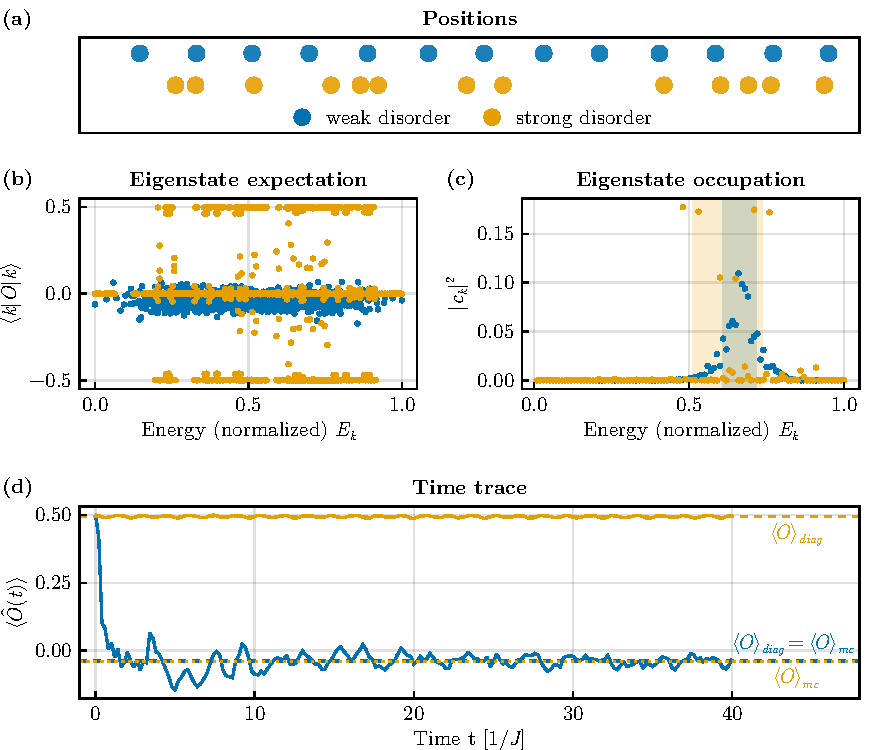
\includegraphics{gfx/part1/ETH-thermalization}
	\caption{Comparison thermalizing and non-thermalizing system using a long-range Heisenberg model (cf. \autoref{eq:long-range-on-site-XXZ}) where $\Delta=0.4$,$\alpha=3$ and $h=0$. The spins are randomly positioned as seen in (a). (b) shows the eigenstate expectation values for the observable $2S_z^{(10)}$. (c) shows the eigenstate occupation numbers (binned into 100 bins) w.r.t. the domain-wall state, where the left 7 spins are $\ket{\downarrow}$ and the other 6 are $\ket{\uparrow}$. The shaded region indicates the mean energy and its variance. The time traces of this operator and initial state are shown in (d). Also shown are the respective prediction by the diagonal and microcanonical ensembles.}
	\label{fig:ETH-thermalization}
\end{figure}

However, ETH alone is not enough to ensure thermalization, we also need to demand that the $c_k$ are concentrated in the spectrum around some mean $\bar{E}$. Then we have indeed
\begin{align}
	\braket[1]{O}_{\omega} = O_{mc}(\bar{E}) = \braket[1]{O}_{mc}(\bar{E}),
\end{align}
where $\braket[1]{O}_{mc}(\bar{E})$ denotes the microcanonical ensemble expectation value at mean energy $\bar{E}$, i.e. the average over all eigenstates within a small energy window $[E-\Delta E, E+\Delta E]$. Physically, this restriction just means that one cannot expect extreme cases, e.g. a superposition of some state at low energy and another at high energy, to thermalize. Fortunately, these scenarios are rare. Usually, experiments initialize their systems in some reasonable state, e.g. product states with well-defined physical properties, which will also be concentrated in the spectrum due to ETH. 

We remark that thermalization according to ETH reflects the key features of thermal equilibrium define in the beginning of this section: The precise initial state is irrelevant and the only information needed to describe its equilibrium properties is its average energy (assuming the absence of other conservation laws). In a sense ETH translates the concept of typicality from the classical world into the quantum realm by demanding that every eigenstate itself looks already thermal when probed locally. 
% TODO dynamical perspective?

To conclude this intro, \autoref{fig:ETH-thermalization} shows a comparison of two concrete systems where one thermalizes (blue) and one is subjected to strong disorder which can prohibit thermalization as described in the following sections. The model itself is a long-range Heisenberg model that will be studied throughout whole \autoref{pt:spatial-disorder} but the details are not relevant to recognize the striking difference between the weakly and strongly disordered cases. Panel (b) clearly shows that ETH is not fulfilled, eigenstate expectation values are highly discontinuous for the strongly disordered system. In contrast, for weak disorder they show no real energy dependence for the chosen observable (which is just the $z$-magnetization of a single spin). Similarly, but not as stark is the contrast for the eigenstate occupation numbers, i.e. the $|c_l|^2$, shown in panel (c) for the domain-wall state $\ket{\downarrow}^{\otimes 7}\ket{\uparrow}^{\otimes 6}$. This is a reasonable state and thus we can see that for weakly disordered system the eigenstate occupations cluster in the spectrum. Conversely for the strongly disordered system, they are spread roughly twice as far. Finally, these spectral properties are reflected in the time evolution of the expectation value of the chosen operator: While for thermalizing system the equilibrium value is reached quickly and agrees with the value obtained by the diagonal and microcanonical ensembles, for the non-thermal system the microcanonical prediction is very far from the actual values.

% loss of memory of the initial conditions
% volume law entanglement
% thermal everywhere
% can be described using a few macroscopic parameters corresponding to conserved quantities, e.g. energy, temperature, magnetization, ...
% namedrop Gibbs ensemble?
% effective tool to understand properties of large quantum systems

%
%\subsection{Prethermalization}
%
%review: \cite{moriThermalizationPrethermalizationIsolated2018}

\section{Many-body Localization (MBL)}
\label{sec:MBL}
In 1958 Anderson discovered that a simple particle hopping between sites in a lattice with random on-site potentials can become stuck completely~\cite{andersonAbsenceDiffusionCertain1958}. This of course means that this simple system does not thermalize at all since the memory of the initial state is retained at all times. This scenario is now known as Anderson localization and was the starting point of a whole new branch of research on localization in disordered systems~\cite{imbrieReviewLocalIntegrals2017,abaninRecentProgressManybody2017,parameswaranEigenstatePhaseTransitions2017,abaninManybodyLocalizationThermalization2019,laflorencieEntanglementEntropyLocalization2022,sierantManyBodyLocalizationAge2024}.
It was later generalized to interacting many-body spin systems~\cite{fleishmanInteractionsAndersonTransition1980,baskoMetalinsulatorTransitionWeakly2006,gornyiInteractingElectronsDisordered2005}, where the most studied model is the paradigmatic Heisenberg XXZ chain with random on-site potentials:
\begin{equation}\label{eq:XXZ-onsite}
	H_{XXZ} = J \sum_i \left(S_x^{(i)}S_x^{(i+1)} + S_y^{(i)}S_y^{(i+1)} + \Delta S_z^{(i)}S_z^{(i+1)}\right) + \sum_i h_i S_z^{(i)}
\end{equation}
Here $S_\alpha^{(i)}$ denotes the spin-half operator in direction $\alpha\in\{x,y,z\}$ on site $i$ and $h_i \sim \mathcal{U}[-W,W]$ are independently drawn from a uniform distribution. The width of this distribution $W$ thus regulates the strength of the disorder.

As found in many studies, this model exhibits a crossover from a thermalizing phase into a localized regime at around $W_c \approx 3-4$ for $\Delta=1$~\cite{oganesyanLocalizationInteractingFermions2007,palManybodyLocalizationPhase2010,berkelbachConductivityDisorderedQuantum2010,delucaErgodicityBreakingModel2013,bauerAreaLawsManybody2013,nanduriEntanglementSpreadingManybody2014,luitzManybodyLocalizationEdge2015,serbynCriterionManybodyLocalizationdelocalization2015,barlevAbsenceDiffusionInteracting2015,devakulEarlyBreakdownAreaLaw2015,luitzExtendedSlowDynamical2016,maceMultifractalScalingsManyBody2019,loganManybodyLocalizationFock2019,chandaManybodyLocalizationTransition2020,tarziaManybodyLocalizationTransition2020,sierantPolynomiallyFilteredExact2020}.
This means that at sufficiently strong disorder $W>W_c$, the properties of this model differ dramatically from those of a thermal system: From the spectral perspective, the energy gap statistic changes from the Wigner-Dyson to a Poissonian distribution~\cite{oganesyanLocalizationInteractingFermions2007}, the eigenstates no longer exhibit volume-law entanglement and show area-law entanglement across the whole spectrum instead~\cite{bauerAreaLawsManybody2013,geraedtsManybodyLocalizationThermalization2016}, and ETH is no longer fulfilled~\cite{kimTestingWhetherAll2014,albaEigenstateThermalizationHypothesis2015,mondainiEigenstateThermalizationTwodimensional2016,mierzejewskiEigenstateThermalizationHypothesis2020}. The dynamical flip side of these properties can be summarized by absence of transport paired with very slow growth of entanglement~\cite{znidaricManyBodyLocalization2008,bardarsonUnboundedGrowthEntanglement2012,nanduriEntanglementSpreadingManybody2014,kiefer-emmanouilidisEvidenceUnboundedGrowth2020,luitzThereSlowParticle2020,huangExtensiveEntropyUnitary2021,chavezUltraslowGrowthNumber2023}.
In short, the system exhibits an emergent integrability although it appears to be a fully interacting model at first glance!
\FIXME{This emergent integrability is probably a bit of a logical leap...}

\subsection{L-bit picture}

\begin{figure}[h!]
	\centering
	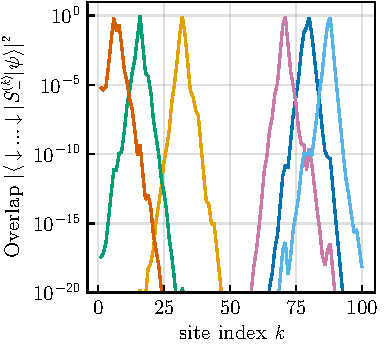
\includegraphics[]{part1/single-spin-localization-xxz}
	\caption{Real-space structure of a couple of eigenstates of the XXZ chain with random on-site potentials (cf. Eq.~\ref{eq:XXZ-onsite}) in the single excitation sector with $W=15$. The exponential tails are clearly visible.}
	\label{fig:xxz-singlespin-exponential-tails}
\end{figure}

This perspective of a many-body localized system as an effectively integrable model unifies the observation made above. It means we can find a basis transformation to write the Hamiltonian in terms of mutually commuting, quasi-local, conserved operators $\tau^{(i)}$, called "local integrals of motion" (LIOM) or "l-bits" such that~\cite{serbynLocalConservationLaws2013,swingleSimpleModelManybody2013,husePhenomenologyFullyManybodylocalized2014}
\begin{equation}\label{eq:l-bit-hamiltonian}
	H = \sum_i h_i \tau^{(i)} + \sum_{i,j} h_{i,j} \tau^{(i)}\tau^{(j)} \ldots
\end{equation}
Here quasi-local means that the operator should essentially act on a single site and decay quickly, i.e. exponentially, when moving away from that site. Fig.~\ref{fig:xxz-singlespin-exponential-tails} shows numerical result for a few eigenstates of the single-excitation sector, where we can see the amplitude decaying exponentially. This means the spins are well and truly localized to a single site and an excitation cannot diffuse away.

Considering a system that can be approximated well be a Hamiltonian of the form \ref{eq:l-bit-hamiltonian}, we can see directly that none of the key features of thermalization defined above hold for MBL systems. Since each of the $\tau^{(i)}$ is quasi-local and conserved some memory of the initial state can always be retrieved by local measurements. From this directly follows, that the measurement depends strongly on the choice of subsystem. However, the \emph{independence of microscopic details} is still partially given: The number of parameters grows with system size but only linearly in the number sites as expected for an integrable system. Thus knowledge about the LIOMs is very useful and allows to make computations for large systems!

In general finding these LIOMs is not a trivial task. For models with random on-site potentials like Eq.~\ref{eq:XXZ-onsite} one can guess that $\tau^{(i)}\approx S_z^{(i)}$ (see e.g.~\cite{adamiStructuralPropertiesLocal2022}) but for more complicated models like the long-range, bond-disordered system considered in the following chapters, it is not as obvious. While there exist different numerical schemes to compute LIOMs~\cite{chandranConstructingLocalIntegrals2015,mierzejewskiIdentifyingLocalQuasilocal2015,mierzejewskiApproximateConservationLaws2015,thomsonLocalIntegralsMotion2021,adamiStructuralPropertiesLocal2022}, we want to focus on gaining insight using an analytical approach falling under name of strong disorder renormalization group or real-space renormalization group (RSRG)~\cite{dasguptaLowtemperaturePropertiesRandom1980,fisherRandomAntiferromagneticQuantum1994,igloiStrongDisorderRG2005,voskManybodyLocalizationOne2013,voskTheoryManyBodyLocalization2015,igloiStrongDisorderRG2018}.

%challenges to observe MBL \cite{abaninDistinguishingLocalizationChaos2021,sierantChallengesObservationManybody2022}

%Still number entropy can grow albeit very slowly\cite{kiefer-emmanouilidisEvidenceUnboundedGrowth2020,chavezUltraslowGrowthNumber2023}
%
%Entanglement entropy similarly\cite{bardarsonUnboundedGrowthEntanglement2012}, proven later\cite{huangExtensiveEntropyUnitary2021}

%Interactions can help\cite{huangInteractionenhancedManybodyLocalization2024}

%\subsection{MBL in the presence of long-range interactions}
\subsection{MBL in long-range, bond-disordered systems}
Considering the mental model for MBL describe above which is caused by random on-site potentials, it is natural to assume that stronger interactions, and more long-range interactions in particular, should be detrimental to localization. Indeed there are heuristic arguments for long-range versions of Eq.~\ref{eq:XXZ-onsite}:
\begin{equation}\label{eq:long-range-on-site-XXZ}
	H = \sum_{i,j} \frac{J_{ij}}{|r_i-r_j|^\alpha} \left(S_x^{(i)}S_x^{(j)} + S_y^{(i)}S_y^{(j)} + \Delta_{ij} S_z^{(i)}S_z^{(j)}\right) + \sum_i h_i S_z^{(i)},
\end{equation}
where $|J_{ij}|=O(1)$, $r_i$ are the locations of the spins and $\alpha$ regulates the spatial decay of the interaction. These arguments then count the number of possible \emph{resonances} for a spin. In this context, two spins $i$ and $j$ are in resonance if their coupling $J_{ij}$ is larger than the energy difference $|h_i-h_j|$ due to the random potentials.
Given a system with spatial dimension $d$, resonance counting rules out localization if $\alpha \leq 2d$ for systems with $|\Delta_{ij}| >0$~\cite{burinEnergyDelocalizationStrongly2006,yaoManyBodyLocalizationDipolar2014,burinManybodyDelocalizationStrongly2015,gutmanEnergyTransportAnderson2016} or $\alpha \leq 1.5d$ in the case of an XX model, i.e. $\Delta=0$~\cite{burinLocalizationRandomXY2015}. Later numerical works supported these predictions by numerically studying systems of $< 40$ spins~\cite{schifferManybodyLocalizationSpin2019,safavi-nainiQuantumDynamicsDisordered2019,yousefjaniMobilityEdgeLongrange2023}.

%Powerlaw with random on-site potentials chain:\\ \cite{safavi-nainiQuantumDynamicsDisordered2019} confirm MBL using dynamics, half-chain entanglement entropy grows with $1/\alpha$. Different critical $\alpha_c$ for XX ($\alpha_c\sim1$) and XXX ($\alpha_c\sim2$). \\
%\cite{schifferManybodyLocalizationSpin2019} confirm MBL using spectral indicators (half-chain entropy, level spacing ratio, variance of HCE). Find $\alpha_c \approx 1.16\pm0.17$. Mobility edge found in\cite{yousefjaniMobilityEdgeLongrange2023}.

\begin{figure}[htb]
	% TODO
	\centering
	\includegraphics[width=0.6\textwidth]{example-image-a}
	\caption{Maybe schematic of the resonance counting? Take from yao paper (with permission)?}
\end{figure}


Conceptually, these works continue the line of thought of random on-site potentials as source of MBL and generalize to power-law interactions with random coefficients. However, there is also a complementary approach, where MBL is caused solely by disordered interactions, e.g. models like
\begin{equation}\label{eq:bond-disordered-XXZ}
	H = \sum_{i} J_{i} \left(S_x^{(i)}S_x^{(i+1)} + S_y^{(i)}S_y^{(i+1)} + \Delta_i S_z^{(i)}S_z^{(i+1)}\right),
\end{equation}
where the $J_{i}$ are independently drawn from some distribution. These bond-disordered models are usually tackled by the real-space renormalization group (RSRG) technique (see~\cite{igloiStrongDisorderRG2005,parameswaranEigenstatePhaseTransitions2017,igloiStrongDisorderRG2018,monthusStrongDisorderRenormalization2018} for reviews). Originally, RSRG was used to find the ground state properties of bond-disordered systems~\cite{dasguptaLowtemperaturePropertiesRandom1980,bhattScalingStudiesHighly1982,fisherRandomTransverseField1992,fisherRandomAntiferromagneticQuantum1994,fisherCriticalBehaviorRandom1995} and later generalized to also compute dynamical properties~\cite{voskManybodyLocalizationOne2013,voskDynamicalQuantumPhase2014,masonTimedependentRealspaceRenormalizationGroup2019,ruggieroQuantumInformationSpreading2022} or study excited states~\cite{pekkerHilbertGlassTransitionNew2014,vasseurQuantumCriticalityHot2015,vasseurParticleholeSymmetryManybody2016}.

The general principle of the RSRG approach is to iteratively eliminate the strongest bond of the system by freezing the spins sharing this bond into one of the eigenstates of their interaction Hamiltonian and deriving new couplings for surrounding spins perturbatively. This is a good approximation, if the system is sufficiently disordered thus that the strongest bond dominates all other couplings in its vicinity. Interestingly, the elimination step \emph{increases} the disorder in the system, such that each successive elimination makes less and less error~\cite{fisherRandomAntiferromagneticQuantum1994}. Thus, the system's coupling distribution flows towards the \emph{infinite randomness fixed point} where the elimination step becomes exact and the coupling distribution converges to a power-law distribution. This line of work culminated in a general theory of the MBL transition for these one-dimensional, bond-disordered, model with nearest neighbor interactions~\cite{voskTheoryManyBodyLocalization2015}.

\FIXME{More detail on elimination process? Less on IRFP? Latter is fine probably}


\begin{figure}[htb]
	% TODO
	\centering
	\includegraphics[width=0.8\textwidth]{example-image-a}
	\caption{Schematic of RSRG elimination}
\end{figure}

Generalizing nearest-neighbor, bond-disordered models to power-law interactions does not significantly change the story from the perspective of the RSRG approach and localization is predicted to persist even without on-site potentials~\cite{moureManyBodyLocalizationTransition2015,moureDisorderedQuantumSpin2018,kutlinRenormalizationLocalizationSmall2020}. This causes tension with the resonance counting arguments which predict the total absence of localization, because without on-site potentials every spin is considered in resonance with every other spin.
Numerical studies in small systems confirmed the presence of a localization crossover~\cite{mohdebEntanglementPropertiesDisordered2020,mohdebExcitedEigenstateEntanglementProperties2022,mohdebGlobalQuenchDynamics2023}. 
% is it true MBL? different phenomenology -> e.g. aramthottilPhenomenologyManybodyLocalization2024
In this thesis, we aim to contribute to this situation with the support of a Rydberg-based quantum simulator, which we introduce in the next section.
 
\FIXME{should probably cite \cite{nandkishoreManyBodyLocalized2017} somewhere}

\FIXME{Mention the whole avalanche thermalization, MBL does not exist debate somewhere}
% "Many body localization with long range interactions" fermionic system -> use bosonization
% very critical of the perturbative resonance counting arguments

%key difference: power-law interactions and random positions create much greater variance of coupling strengths

% relevant for experiment
% This thesis first studies the applicability of RSRG in the context of the type of disorder the experiment has
% then uses it to explain observable signatures to address the question whether the experiment thermalizes or not (on experimentally accessible timescales)


% juhaszRandomTransversefieldIsing2014 LR-TFIM on-site disorder	
% monthusDysonHierarchicalQuantum2015 LR-TFIM on-site disorder
% modakManybodyDynamicsLongrange2020,modakManybodyLocalizationLongrange2020a - fermionic hopping with on-site potential
%While localization in bond-disordered models does not cause tension to the results from resonance counting for nearest neighbor interaction due to the limited interaction range. However most quantum simulation experiments based on atoms or molecules feature power-law interactions due to the electronic interactions. 

%Recently, these branches of bond-disordered systems and long-range interactions came into contact due to the study of long-range models without on-site disorder. While resonance counting arguments would predict the complete absence of localization, since all spins are considered to be resonant, numerical studies showed signs of localization.

%In this context, the first part of this thesis first studies localization in a power-law interacting XXZ  model with specific disorder arising from random positions subject to a blockade condition. Our main focus lies not on the question whether this model exhibits true MBL in the limit of infinite system size and/or at very late times. Rather, we aim to use MBL as a practical tool to gain insight in the dynamics and properties of the model at experimentally accessible scales. For this, we first employ numerical methods to establish that small systems 

%This is a different regime than what I study where the main disorder does not stem from random potentials but is due to widely varying interaction strengths. To make this difference clear, I note that without random fields, these early works claim MBL to be impossible, as any spin is resonant with every other spin. However, RSRG tells us that each spin effectively on interacts with its \emph{strongest} resonant partner. Their fast interaction then effectively decouples the pair from the rest of the spins. That's why this resonance counting is not relevant for localization for truly bond-disordered systems and raises the question about possible differences between random field models with some random long-range interaction and bond-disordered models with some random fields.


%Interestingly, even in ordered systems with very long-range interaction $\alpha<1$ ETH is violated~\cite{sugimotoEigenstateThermalizationLongRange2022,chengManybodyLocalizationClean2023}.

%heuristic resonance counting, no MBL for $\alpha\leq d$ in XXZ or Anderson model \cite{burinEnergyDelocalizationStrongly2006} with somewhat mixed behavior for $\alpha\leq 2d$ (Anderson localization at zero temperature, other pair forms for Yao XXZ). 
%
%Refined by  for XX model to $\alpha > \frac{3d}{2}$.





%

%
%\subsection{Localization in long-range, bond-disordered systems}
%RSRG and schrieffer-wolff trafo
%
%Long-range bond-disorder:
%\cite{mohdebEntanglementPropertiesDisordered2020,mohdebExcitedEigenstateEntanglementProperties2022,mohdebGlobalQuenchDynamics2023}
%
%\begin{figure}[htb]
%	% TODO
%	\centering
%	\includegraphics[width=0.8\textwidth]{example-image-a}
%	\caption{Schematic of pair localization}
%\end{figure}


%\subsection{Does MBL exist?}
%Existence proof (TFIM): \cite{imbrieManyBodyLocalizationQuantum2016}
%
%However, MBL might be finite size
%
%Avalanche thermalization
%
%\begin{figure}[htb]
%	% TODO
%	\centering
%	\includegraphics[width=0.8\textwidth]{example-image-a}
%	\caption{Schematic of the avalanche thermalization.}
%\end{figure}